\subsection{SP-24 (PSI)}
ISO/OSI model, enkapsulace a dekapsulace posílaných dat, princip IP adresace. Linková vrstva, podvrstvy LLC. MAC, síťová zařízení, princip přepínání. Virtuální sítě (VLAN). Síťová vrstva, směrovače, princip směrování, protokoly IPv4 a IPv6, statické a dynamické směrování.

\subsubsection*{OSI Model}
\begin{itemize}
	\item Open System Interconnection
	
	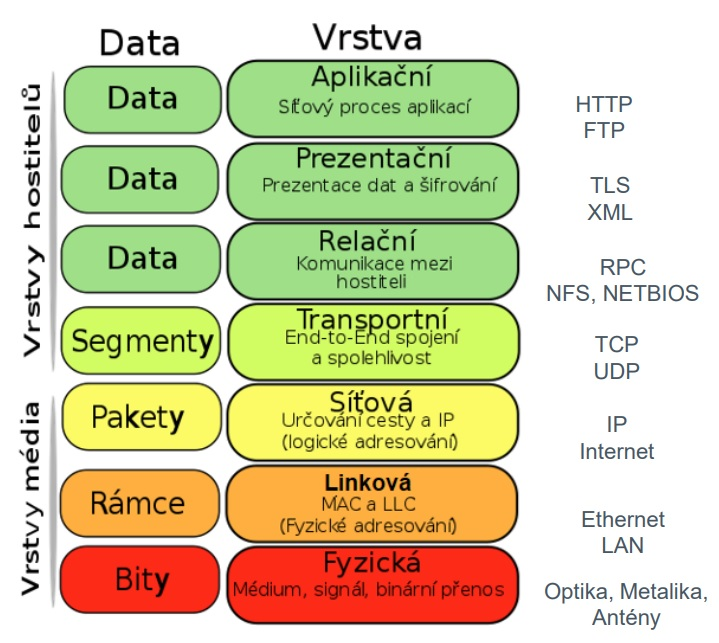
\includegraphics[width=0.6\textwidth]{img/SP-24_0.jpg}
	
	\item Aplikační vrstva --- protokoly pro komunikaci mezi aplikacemi, přenáší se data a zajímá nás význam
	\item Prezentační vrstva --- formátování a prezentace dat, šifrování, přenáší se data a zajímá nás struktura
	\item Relační vrstva --- logické rozhraní pro aplikace, RPC, sdílení filesystému, přenáší se data
	\item Transportní vrstva --- data jsou rozložena na segmenty, typicky protokol transportní vrstvy přidá nějakou hlavičku, posílá se z portu na port, řeší se E2E spojení a spolehlivost
	\item Síťová vrstva --- segmenty vyšších vrstev rozděleny na pakety, posílají se na síťovou adresu (IP)
	\item Linková vrstva --- pakety rozděleny na rámce (frames), opět přidána hlavička, posílá se na linkovou adresu (MAC)
	\item Fyzická vrstva --- převod rámců na bity a posílání přes médium (kabel, vzduch)
	
\end{itemize}

\textbf{TCP/IP model}
\begin{itemize}
	\item pouze 4 vrstvy: aplikační (první 3 OSI), transportní, internetová a síťová (spodní 2 OSI)
\end{itemize}

\subsubsection*{IP adresace}
\begin{itemize}
	\item IPv4 adresa --- 4 byty
	\item stanice v IPv4 síti se sdružují do podsítí
	\begin{itemize}
		\item adresní rozsah sítě --- skupina všech IP adres, které patří do stejné sítě
		\item maska --- určuje rozsah, je stejně dlouhá jako IP adresa, používá se prefixová notace (aaa.bbb.ccc.ddd /mm --- mm je počet bitů masky od začátku, které jsou 1)
		\item adresa sítě --- získá se z adresy nějakého zařízení v síti operací AND s maskou --- nejnižší adresa v daném rozsahu
		\item broadcast --- nejvyšší adresa z rozsahu
	\end{itemize}
\end{itemize}

\subsubsection*{Linková vrstva}
\begin{itemize}
	\item přenášení dat v rámci lokální (LAN) sítě
	\item základní přenášená jednotka je rámec (frame)
	\item skládá se z 2 podvrstev: MAC a LLC
	\item MAC:
	\begin{itemize}
		\item Medium Access Control
		\item zajišťuje přístup k médiu (fyzické vrstvě)
		\item řeší fyzickou adresaci pomocí MAC adres
		\item filtrování MAC adres
		\item plánování rámců do front  a jejich odesílání
		\item VLAN
		\item svázána s konkrétní technologií fyzické vrstvy
		\item řeší sdílený přístup k médiu (multiplex --- řešení kolizí --- časový, frekvenční, kódový, prostorový)
		\item další metody přístupu k společnému médiu --- Carrier Sense Multiple Access (CSMA (-/CD/CA))
		
		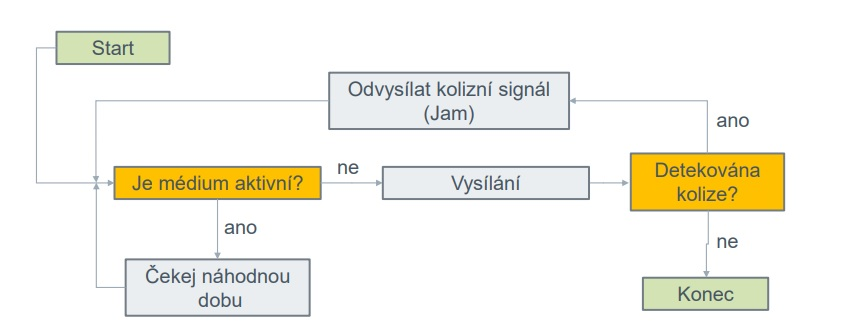
\includegraphics[width=0.6\textwidth]{img/SP-24_1.jpg}
	\end{itemize}
	\item LLC:
	\begin{itemize}
		\item Logical Link Control
		\item umožňuje existenci různých protokolů nad společnou MAC vrstvou
		\item řízení toku a kontrola chyb
		\item rozdělení toku dat z vyšších vrstev do rámců, určení velikosti rámce a jeho zakončení
		\item zajištění doručení dat --- potvrzovací schémata
		\begin{itemize}
			\item jednotlivé potvrzování (stop \& wait)
			\item selective repeat
			\item Go-Back-N
			\item klouzavé okénko
		\end{itemize}
	\end{itemize}
	\item Zařízení na linkové vrstvě:
	\begin{itemize}
		\item pracují s rámci
		\item obecný formát: hlavička, data, konec rámce (obsahuje např kontrolní součet)
		\item switch --- porty, které mají buffery --- přepínací tabulka, aby věděl kam posílat dál, switch se učí --- různé režimy přeposílání (store and forward, cut through, fragment free)
		\item bridge
	\end{itemize}
	\item broadcastová doména --- množina stanic dané sitě, kterým je doručen rámec s broadcastovou adresou
	\item v síti nesmí být smyčky, lze odstranit přes SPT (spanning tree protocol), udělá kostru
	\item MAC adresa: 6 bytů, první 3 identifikují výrobce
	
	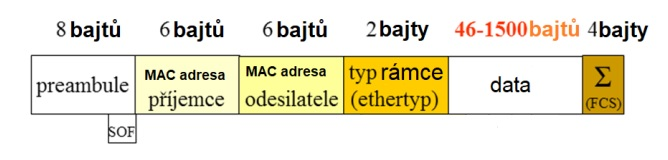
\includegraphics[width=0.6\textwidth]{img/SP-24_2.jpg}
\end{itemize}

\subsubsection*{VLAN}
\begin{itemize}
	\item každý port na switchi se dá zařadit do VLAN
	\item trunk port podporuje více (všechny) VLAN
	\item trunkem chodí označené rámce (tagged), k workstations chodí neoznačené
	\item pro přeposílání dat mezi VLAN se musí chodit přes router
	\item VLAN může být dána jak portem, tagem, tak MAC adresou nebo protokolem vyšší úrovně
\end{itemize}

\subsubsection*{Síťová vrstva}
\begin{itemize}
	\item doručuje data jak v lokální síti, tak mezi sítěmi
	\item schémata IP adresace: prefixová a dle třídy

	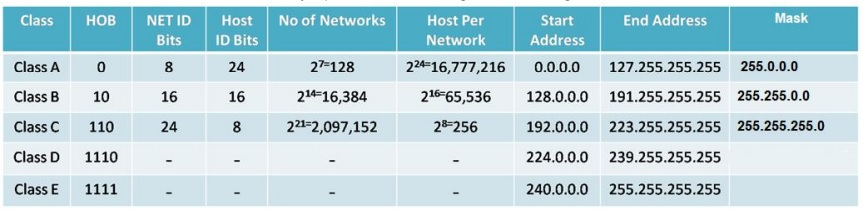
\includegraphics[width=0.8\textwidth]{img/SP-24_3.jpg}	
	
	\item speciální rozsahy:
	\begin{itemize}
		\item privátní (10.0.0.0/8, 172.16.0.0/12, 192.168.0.0/16)
		\item link-local (169.254.0.0/16)
		\item loop-back (127.0.0.0/8)
		\item multicast (224.0.0.0/4)
	\end{itemize}
	
	\item hlavička IP paketu:
	
	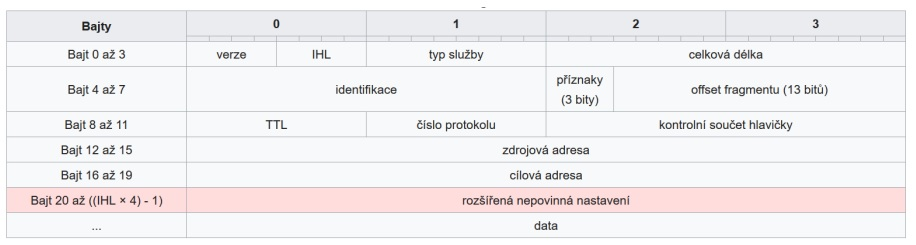
\includegraphics[width=0.8\textwidth]{img/SP-24_4.jpg}
	
	\item princip směrováni:
	\begin{itemize}
		\item směrování (routing) --odeslání konkrétního paketu prostřednictvím zvoleného síťového rozhraní na základě cílové IP adresy paketu
		\item provádí router
		\item podle toho, zda cílová adresa patří do sítě routeru se paket buď pošle cílové stanici, nebo dalšímu routeru podle směrovací tabulky
		\item směrovací tabulka má záznamy o sítích, a jakým způsobem se k nim dostat (kam a jak poslat paket)
		\item ruční zadání informací do tabulky = statické směrování
	\end{itemize}
	\item NAT (Network Address Translation) --- překlad adres na routeru z veřejné (adresa routeru) na privátní (za routerem, adresy v soukromé síti)
	\item ICMP (Internet Control Message Protocol) --- utility ping a tracert/traceroute
	\item ARP (Address Resolution protocol) --- chceme poslat paket na IP adresu, ale neznáme MAC adresu, tak se zeptáme přes MAC broadcast "kdo má tuto IP" ... cíl odpoví už ne přes broadcast že on má tuto adresu, tedy uložíme do ARP table
	\item DHCP (Dynamic Host Control Protocol) --- dynamické nastavení IP adresy a nastavení sítě pro stanici (4 zprávy, vše broadcast)
\end{itemize}

\subsubsection*{Směrování}
\begin{itemize}
	\item typy směrování:
	\begin{itemize}
		\item Redundantní --- existuje více cest do cíle
		\item symetrické --- cesta tam je stejná jako zpět
		\item asymetrické --- cesty tam a zpět se liší
		\item proaktivní --- používá směrovací tabulky, předpočítá/ví cestu do cíle (běžně v počítačových sítích)
		\item reaktivní --- zjišťuje cestu až na základě žádosti (např. v mobilních sítích)
	\end{itemize}
	\item Dynamické směrování --- algoritmy:
	\begin{itemize}
		\item Distance Vector algoritmy (např. RIP --- routing information protocol) --- routery si vymění navzájem info o vzdálenosti všech sousedů, dělají to i za běhu, tedy + router i - router, vzdálenost je pouze počet routerů v cestě
		\item Link-State algoritmy (např. OSPF) --- sestaví graf sítě i s ohodnocením hran (linkstate udaná správcem sítě)
		\item Path Vector algoritmy (např. BGP) --- routery si vyměňují celé cesty ke konkrétním cílům
	\end{itemize}
\end{itemize}

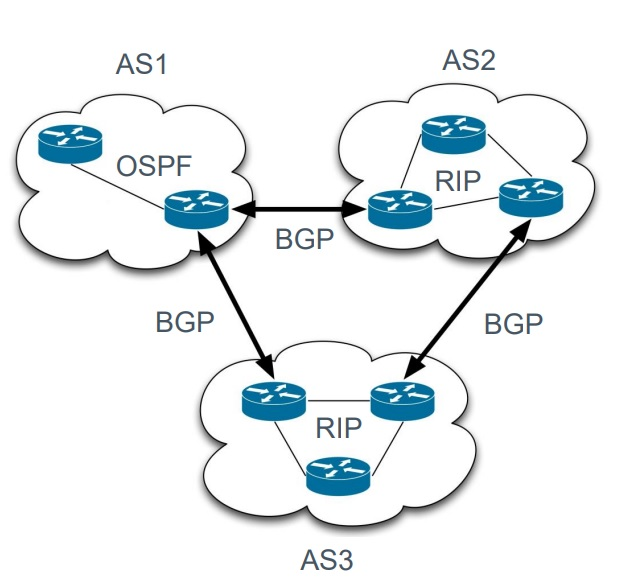
\includegraphics[width=0.6\textwidth]{img/SP-24_5.jpg}

\subsubsection*{IPv6}
\begin{itemize}
	\item umožňuje zřetězit hlavičky, hlavička je jednodušší
	\item 128b adresy (16B)
	\item není potřeba NAT
	\item umožňuje objevování sousedů, efektvnější seměrování, ...
\end{itemize}